\LARGE{ \textbf {Лекция №11}}\\
\Large{ \textbf {Основные параметры счетчиков}}\\

М - модуль счета или коэффициент пересечения.\\
Модуль счета - число устойчивых состояний счетчика, т.е. предельное число импульсов,
которое могут быть подсчитаны счетчиком.

$M = 2^n $, где  n число разрядов для двоичных.\\
$ 0 \to 1 \to 2 \to ... \to 2^n-2 \to 2^n -1  $\\
$N = M^n  -1 $\\
$M = 10  n = 3 N = 10^3 - 1 = 999$\\
$M = 2  n = 3 N = 2^3 - 1 = 7$\\


\textbf{Основные динамические параметры счетчиков}\\
Максимальная частота посупления импульса на вход счетчика - это величина обратная
минимальному допостимому интервалу времени между 2 счетными импульсами.
При котором не происходит потеря счета.
$T > \frac{1}{t_cr}$\\
Время установки кода счетчика - минимальный временной интервал между момемнтом поступления
счетного импульса и моментом установления кода счетчика.\\

Для счетчиков построенных на двуступеньчатых триггерах время установки определяется максимальным
временным интервалом между моментом окончания счетного импульса и моментом окончания переходных процессов во всех разрядах счетчика.\\
При использовании триггеров с динамическим управлением запись время установки кода счетчика
описывается от фронта входного сигнала вызывающего переключение триггеров.\\
\textbf{Синтез синронных счетчиков с паралелльным переносом с произвольным модулем счета.}\\
Задача - построить счетчик.\\
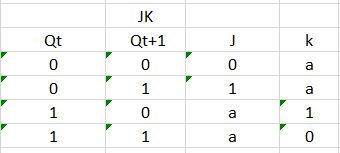
\includegraphics{38}\\
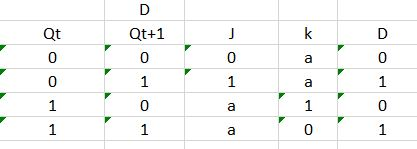
\includegraphics{39}\\

\begin{enumerate}
  \item В синхронных счетчиках входный сигнал подается на входы С всех триггеров.
  \item Определение числа разрядов счетчика: $n = ]log_2 M[$ скобки - прближение до ближайшего целого числа.
  $M =10 \quad n = ]log_2 10 [~]3,16[ = 4 $
  \item Выбирается тип триггеров, как правило JK или D.
  Как правило JK - потому что легче схеме.
  \item Для каждого типа триггера существует своя таблица перехода.
  \item Составляется таблица переходов - позволяет определить функции управляющих сигналов для входов J,K всех триггеров в виде:
  $ J_i^t = f_i(Q_4,Q_3,Q_2,Q_1)^t$  $ K_i^t = \phi_i(Q_4,Q_3,Q_2,Q_1)^t$
  Эти функции должны быть минимизированы. Метод карт карно.
\end{enumerate}
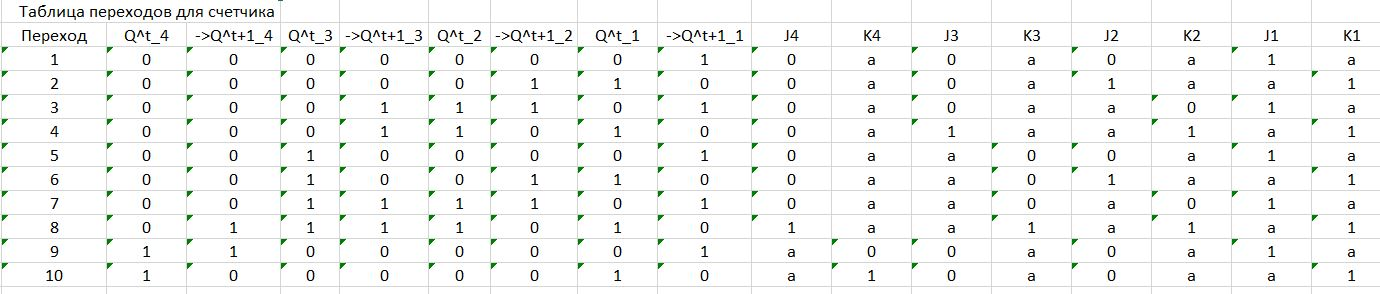
\includegraphics[width=\linewidth,height=\textheight/4]{40}\\
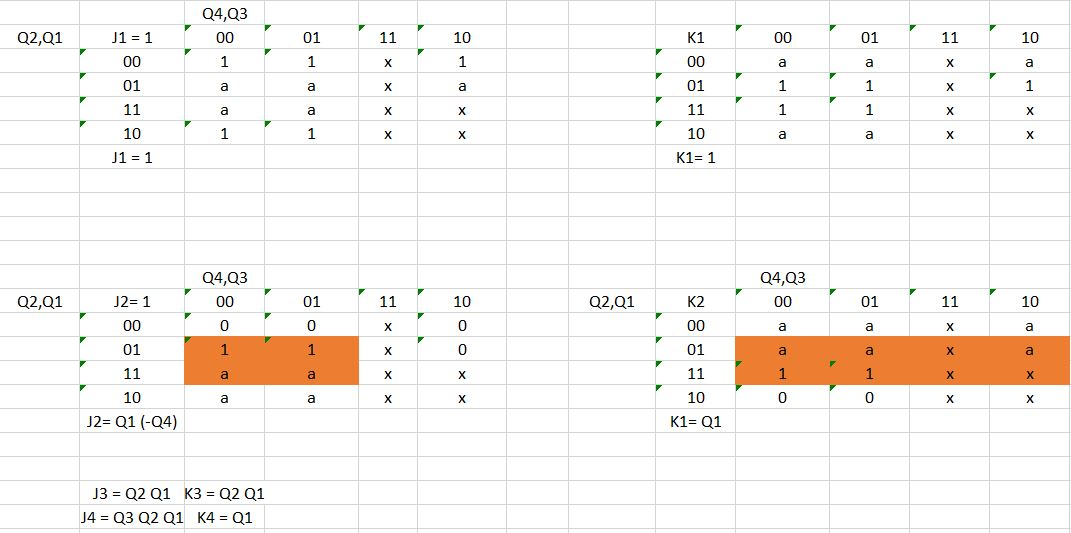
\includegraphics[width=\linewidth]{41}\\
Перключение триггеров происдит по всем разрядам одновременно.
Время срабытвания триггера - время установки кода счтчика.\\
$T \geq t_4^{T2} + t_{yst} t_{zd.sr.}$\\


Функциональные узлы .\\
\textbf{Дешифраторы.}
Дешифратор - функциональный узел, преобразующий каждую комбинацию входных сигналов в информационный
сигнал на выходе номер которого соответсвует десятичному эквиваленту входного кода.
Число выходов дешифратора равно числу разрешенных входных сигналов. $ n -> \quad K \leq 2^n$ Если  $K = 2^n$ - полный,  $K < 2^n$ - неполный.

Полный дешифратор:

$\begin{cases}
  y_0 = \overline{x}_1 \overline{x}_2 ... \overline{x}_{n-2} \overline{x}_{n-1} \overline{x_n} \\
  y_1 = \overline{x}_1 \overline{x}_2 ... \overline{x}_{n-2} \overline{x}_{n-1} {x_n}\\
  y_2=  \overline{x}_1 \overline{x}_2 ... \overline{x}_{n-2} x_{n-1} \overline{x_n}\\
  y_3=  \overline{x}_1 \overline{x}_2 ... \overline{x}_{n-2} x_{n-1} {x_n} \\

\end{cases}$
$DC $\\
Основные параметеры дешифраторов.\\
Число входов n.\\
Число выходов K.\\
Входные,выходные токи 0,1.
Напряжение
Мощность или ток потребления \\

Динамичские параметры.\\
Время задержки распространения из 0 в 1. Наоюорот.\\

Существует 3 основных способа построения дешифраторов: линейный, парамидальный, ступеньчатый.
